\documentclass[tikz, border=10pt]{standalone}
\usepackage[utf8]{inputenc}
\usepackage[T1]{fontenc}
\usetikzlibrary{shapes.geometric, arrows.meta, positioning, fit, backgrounds, calc, shadows}

% --- USC Brand Colors (matching EMCH 501 formatting) ---
\definecolor{USC_Garnet}{HTML}{73000A}       % Primary maroon/garnet
\definecolor{USC_Sandstorm}{HTML}{FFF2E3}    % Cream background
\definecolor{USC_Black90}{HTML}{565656}      % Dark gray
\definecolor{USC_Black10}{HTML}{ECECEC}      % Light gray background
\definecolor{USC_Honeycomb}{HTML}{65780B}    % Olive/honeycomb green

% Derived colors for the diagram
\definecolor{userColor}{HTML}{73000A}        % USC Garnet for user actions
\definecolor{sysColor}{HTML}{565656}         % USC Black90 for system processes
\definecolor{laneUser}{HTML}{FFF2F2}         % Very light garnet tint for user lane
\definecolor{laneSys}{HTML}{ECECEC}          % USC Black10 for system lane
\definecolor{lineColor}{HTML}{73000A}        % USC Garnet for arrows
\definecolor{decisionColor}{HTML}{65780B}    % USC Honeycomb for decisions

\begin{document}

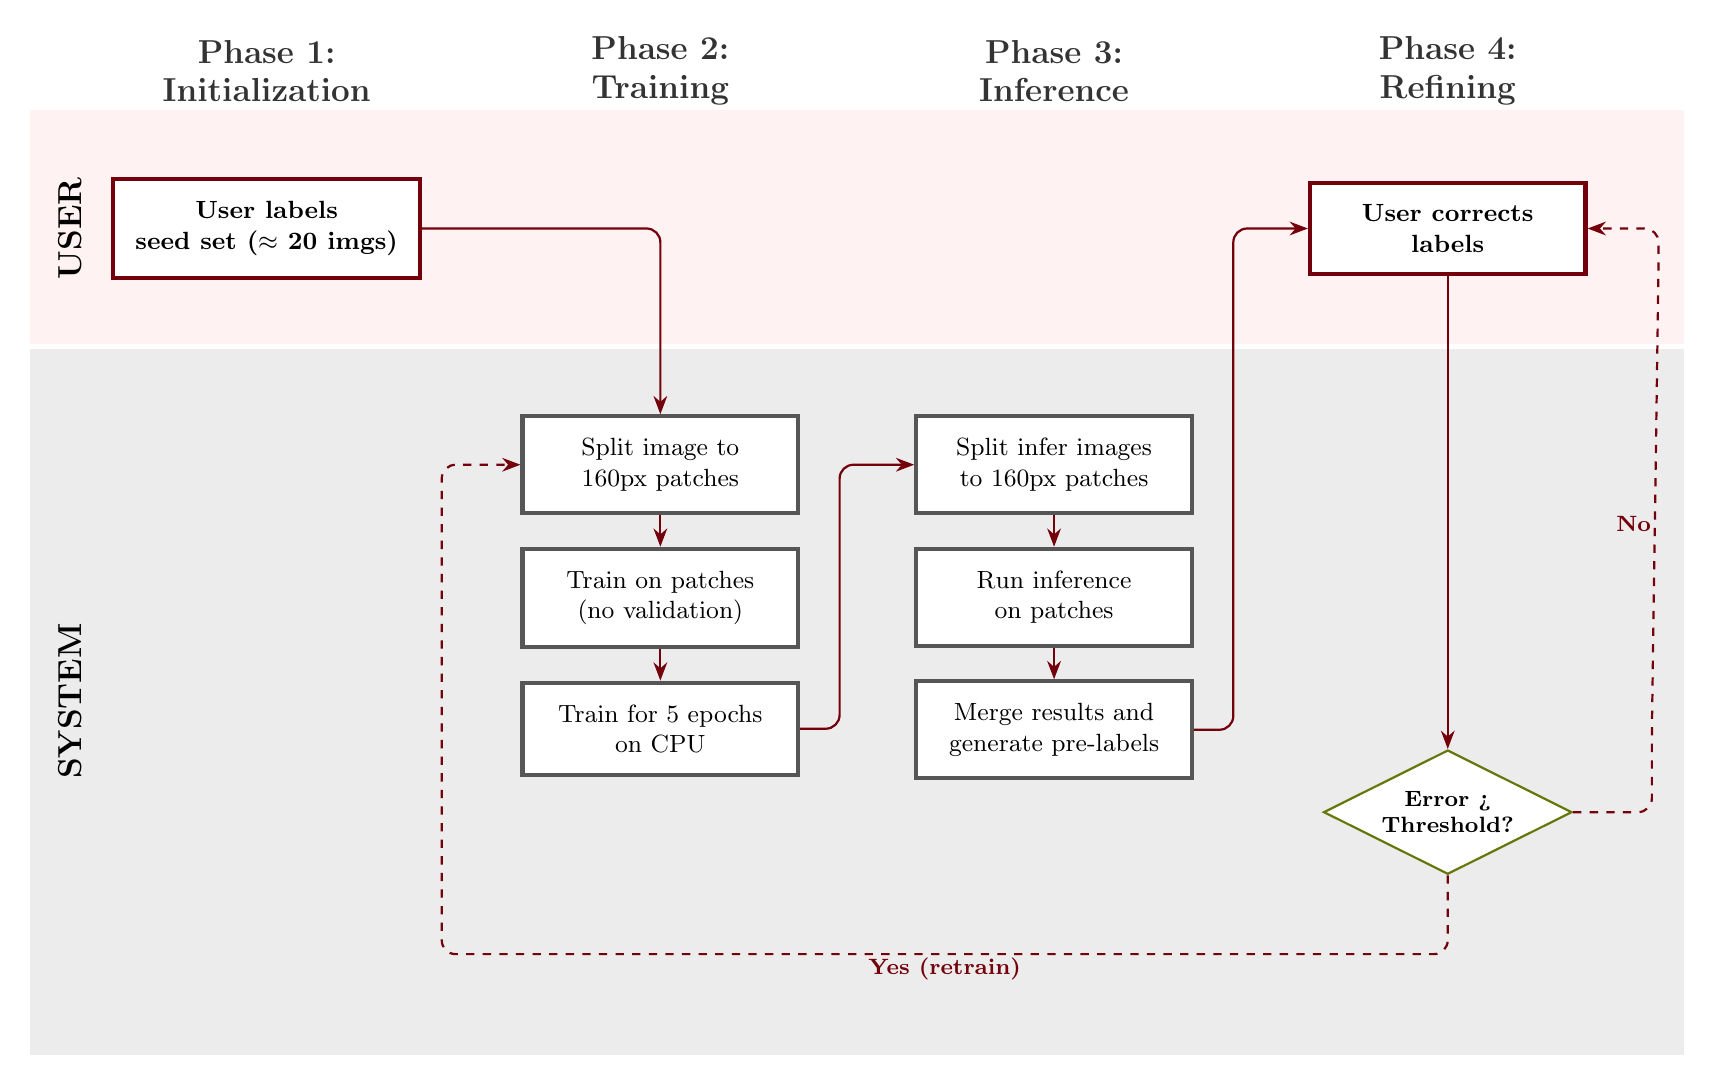
\begin{tikzpicture}[
    node distance=1.0cm and 1.5cm,
    % Box Styles
    base/.style={
        draw=none,
        sharp corners,
        align=center,
        font=\small,
        minimum width=3.5cm,
        inner sep=8pt
    },
    userBox/.style={
        base,
        draw=userColor,
        line width=1.5pt,
        fill=white,
        text=black,
        font=\small\bfseries
    },
    sysBox/.style={
        base,
        draw=sysColor,
        line width=1.5pt,
        fill=white,
        text=black
    },
    decision/.style={
        diamond,
        aspect=2,
        draw=decisionColor,
        thick,
        fill=white,
        text=black,
        align=center,
        font=\footnotesize\bfseries,
        inner sep=2pt
    },
    % Line Styles
    connector/.style={
        ->,
        thick,
        color=lineColor,
        >=Stealth,
        rounded corners=5pt
    },
    loopLine/.style={
        connector,
        dashed
    },
    % Text Styles
    phaseHeader/.style={
        font=\large\bfseries\color{black!80},
        align=center
    },
    laneLabel/.style={
        font=\large\bfseries\color{black},
        rotate=90,
        anchor=center
    }
]

    % --- GRID SETUP & SWIMLANES ---
    % We define coordinates for the grid to keep things aligned
    
    % Coordinates for Columns (Phases)
    \coordinate (c1) at (0,0);
    \coordinate (c2) at (5,0);
    \coordinate (c3) at (10,0);
    \coordinate (c4) at (15,0);

    % Coordinates for Rows (Lanes)
    \coordinate (rUser) at (0, 0);
    \coordinate (rSys) at (0, -4);

    % Draw Swimlane Backgrounds
    \begin{scope}[on background layer]
        % User Lane
        \fill[laneUser] (-3, 1.5) rectangle (18, -1.5);
        \node[laneLabel] at (-2.5, 0) {USER};
        
        % System Lane
        \fill[laneSys] (-3, -1.5) rectangle (18, -10.5); % Extended depth for system stack
        \node[laneLabel] at (-2.5, -6) {SYSTEM};
        
        % Separator
        \draw[white, line width=2pt] (-3, -1.5) -- (18, -1.5);
    \end{scope}

    % --- PHASE 1: INITIALIZATION ---
    \node[phaseHeader] at (0, 2) {Phase 1:\\Initialization};
    
    \node[userBox] (seed) at (0,0) {User labels\\seed set ($\approx$ 20 imgs)};

    % --- PHASE 2: TRAINING ---
    \node[phaseHeader] at (5, 2) {Phase 2:\\Training};
    
    % System Stack for Training
    \node[sysBox] (split1) at (5, -3) {Split image to\\160px patches};
    \node[sysBox, below=0.4cm of split1] (train) {Train on patches\\(no validation)};
    \node[sysBox, below=0.4cm of train] (epoch) {Train for 5 epochs\\on CPU};

    % --- PHASE 3: INFERENCE ---
    \node[phaseHeader] at (10, 2) {Phase 3:\\Inference};
    
    % System Stack for Inference
    \node[sysBox] (split2) at (10, -3) {Split infer images\\to 160px patches};
    \node[sysBox, below=0.4cm of split2] (infer) {Run inference\\on patches};
    \node[sysBox, below=0.4cm of infer] (merge) {Merge results and\\ generate pre-labels};

    % --- PHASE 4: CORRECTION & LOOP ---
    \node[phaseHeader] at (15, 2) {Phase 4:\\Refining};
    
    \node[userBox] (correct) at (15, 0) {User corrects\\labels};
    
    \node[decision, below=6cm of correct] (decide) {Error >\\Threshold?};


    % --- CONNECTIONS ---

    % 1. Initialization -> Training
    \draw[connector] (seed) -| (split1);

    % 2. Internal Training Flow
    \draw[connector] (split1) -- (train);
    \draw[connector] (train) -- (epoch);

    % 3. Training -> Inference
    % (Connecting bottom of training to top of inference stack logically)
    \draw[connector] (epoch.east) -- ++(0.5,0) |- (split2.west);
    \draw[connector] (merge.east) -- ++(0.5,0) |- (correct.west);

    % 4. Internal Inference Flow
    \draw[connector] (split2) -- (infer);
    \draw[connector] (infer) -- (merge);
    \draw[connector] (correct) -- (decide);


    % 6. Correction -> Decision
    % \draw[connector] (correct) -- (decide);

    % 7. THE LOOP (Decision -> Training)
    % If Yes: Loop back to Training
    \draw[loopLine]
        (decide.south) -- ++(0,-1.0) -| node[below,pos=0.25,font=\footnotesize\bfseries,inner sep=1pt]{Yes (retrain)}
        ($(split1.west)+(-1.0,-0.5)$) |- (split1.west);
    
    % 8. Decision -> Continue
    % If No: Continue / Done
    \draw[loopLine] (decide.east) -| ++(1,1.0) -- node[left,pos=0.45,font=\footnotesize\bfseries,inner sep=1pt]{No}
        ($(correct.east)+(0.9,-0.5)$) |- (correct.east);

\end{tikzpicture}
\end{document}